% E10 means and sample standard deviations; successful runs only.
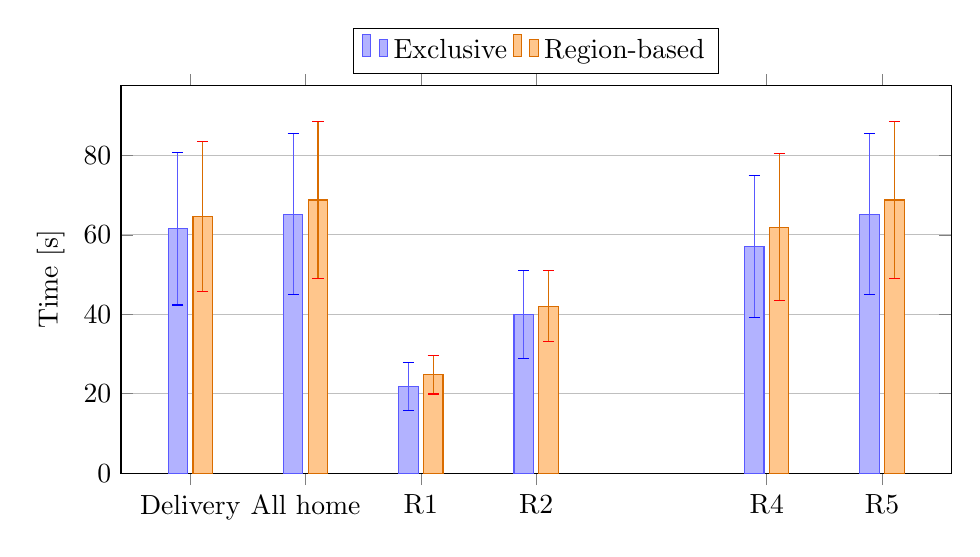
\begin{tikzpicture}
\begin{axis}[ybar,bar width=7pt,width=\linewidth,height=6.5cm,
symbolic x coords={Delivery,All home,R1,R2,R3,R4,R5},xtick=data,ymin=0,ylabel={Time [s]},
legend style={at={(0.5,1.03)},anchor=south,legend columns=2},enlarge x limits=0.1,ymajorgrids=true]
\addplot+[draw=blue!65,fill=blue!30,error bars/.cd,y dir=both,y explicit] coordinates {(Delivery,61.5734) +- (0,19.2392) (All home,65.1480) +- (0,20.2714) (R1,21.8063) +- (0,6.0977) (R2,39.9784) +- (0,11.1377) (R4,57.0611) +- (0,17.8428) (R5,65.1480) +- (0,20.2714)};
\addlegendentry{Exclusive}
\addplot+[draw=orange!85!black,fill=orange!45,error bars/.cd,y dir=both,y explicit] coordinates {(Delivery,64.6191) +- (0,18.8567) (All home,68.7581) +- (0,19.8476) (R1,24.7947) +- (0,4.8689) (R2,42.0508) +- (0,8.8843) (R4,61.9328) +- (0,18.4678) (R5,68.7581) +- (0,19.8476)};
\addlegendentry{Region-based}
\end{axis}
\end{tikzpicture}
